\documentclass[11pt]{report}
\usepackage[utf8]{inputenc}
\usepackage[T1]{fontenc}
 \usepackage{listings}
\usepackage{amsmath}

\usepackage{fancyhdr}
\usepackage{graphicx}
\usepackage{color}
\pagestyle{fancy}


 \lhead{Geoffrey PERRIN - Océane DUBOIS}
 \rhead{}
 \rfoot{}



\definecolor{codegreen}{rgb}{0,0.6,0}
\definecolor{codegray}{rgb}{0.5,0.5,0.5}
\definecolor{codepurple}{rgb}{0.58,0,0.82}
\definecolor{backcolour}{rgb}{0.95,0.95,0.92}

\lstdefinestyle{mystyle}{
    backgroundcolor=\color{backcolour},
    commentstyle=\color{codegreen},
    keywordstyle=\color{magenta},
    numberstyle=\tiny\color{codegray},
    stringstyle=\color{codepurple},
    basicstyle=\footnotesize,
    breakatwhitespace=false,
    commentstyle=\color{codegreen},   
    breaklines=true,
    captionpos=b,
    keepspaces=true,
    numbers=left,
    numbersep=5pt,
    showspaces=false,
    showstringspaces=false,
    showtabs=false,
    tabsize=2,
     morekeywords={mov, push, xor, extern, div, mov, inc, cmp, jne, call, pop, ret,endp, proc, end, dec, add, jb, dd, db, jge,  not, lea, main, public, movzx, imul, shl, sub, jg, neg, test, jle, jns, jnz, and, shr, ja},
   extendedchars=true,
    sensitive=false,
   morecomment=[l];,
    literate= {á}{{\'a}}1 {é}{{\'e}}1 {í}{{\'i}}1 {ó}{{\'o}}1 {ú}{{\'u}}1 {Á}{{\'A}}1 {É}{{\'E}}1 {Í}{{\'I}}1 {Ó}{{\'O}}1 {Ú}{{\'U}}1 {à}{{\`a}}1 {è}{{\`e}}1 {ì}{{\`i}}1 {ò}{{\`o}}1 {ù}{{\`u}}1 {À}{{\`A}}1 {È}{{\'E}}1 {Ì}{{\`I}}1 {Ò}{{\`O}}1 {Ù}{{\`U}}1 {ä}{{\"a}}1 {ë}{{\"e}}1 {ï}{{\"i}}1 {ö}{{\"o}}1 {ü}{{\"u}}1 {Ä}{{\"A}}1 {Ë}{{\"E}}1 {Ï}{{\"I}}1 {Ö}{{\"O}}1 {Ü}{{\"U}}1 {â}{{\^a}}1 {ê}{{\^e}}1 {î}{{\^i}}1 {ô}{{\^o}}1 {û}{{\^u}}1 {Â}{{\^A}}1 {Ê}{{\^E}}1 {Î}{{\^I}}1 {Ô}{{\^O}}1 {Û}{{\^U}}1,
  }

\lstset{style=mystyle}

%Gummi|065|=)
\title{\textbf{TP06/TP07 - Traitement d'image - deuxième partie }
\author{Geoffrey PERRIN \\ Océane DUBOIS\\}
\date{}}

\begin{document}

\maketitle

\newpage

Le but de ce TP est de construire un algorithme permettant de détecter les contours d'un image. Pour ce faire on utilisera la méthode du gradient, qui consiste à réaliser la dérivée de l'intensité des pixels, si on observe un maximum, on considère que c'est un contour.


\begin{figure}[h]
\begin{center}
$
\begin{bmatrix}
-1 & 0 & 1 \\
-2 & 0 & 2 \\
-1 & 0 & 1 
\end{bmatrix}
$
\end{center}
\label{sx}
\caption{Masque de convolution de Sobel Sx}
\end{figure}


\begin{figure}[h]
\begin{center}
$
\begin{bmatrix}
1 & 2 & 1 \\
0 & 0 & 0 \\
-1 & -2 & -1 
\end{bmatrix}
$
\label{sy}
\end{center}
\caption{Masque de convolution de Sobel Sy}
\end{figure}


Pour nous aider à retrouver le gradient des pixels de l'image, on utilisera l'opérateur de sobel qui est composé de 2 masques de convolution Sx et Sy définis par les figures 1 et 2.

Attention, on ne pourra pas appliquer les masques sur la première et dernière ligne de pixel ni sur la première et dernière colone de pixel car le masque dépasserait de l'image. Pour le TP on ignorera cet lignes et colones. 


\section{Calcul des adresses source et destination}

Soit esi contenant l'adresse du premier pixel auquel on applique le masque et edi est l'adresse du premier pixel de l'image de destination (img\_temp2). On stocke dans ebp la taille d'une ligne de pixels.

Ainsi ecx contient la hauteur de l'image, à laquelle on soustrait 2 pour ignorer la première et la dernière ligne.

Esi contient l'adresse du premier pixel de l'image tmp1
Edi contient l'adresse du premier pixel de l'image tmp2
Ebp contient le nombre de pixel sur la ligne d'une image. 

Pour connaitre la taille d'une ligne il suffit de multiplier Ebp par 4(la taille d'un pixel en mémoire).


\section{Contruction de la double itération}

Dans le but d'économiser un registre, ecx contiendra sur la partie haute le compteur de lignes et sur sa partie base le compteur de colones.Ainsi on peut récupérer facilement le comtpeur des lignes dans cx.


\section{Itération sur les lignes}

Au début de la boucle on initialise les bits de poids fort avec ebp -2, pour ignorer les premières et dernièrers lignes. 

A la fin de chaque ligne on soustrait 00010000h à ecx. Lorsque les bits de poids forts de ecx arrivent à 0, on arrête la boucle. Cela signifie qu'on a traité tous les pixels de l'image.

\section{Itération sur les colones}

On place donc dans la partie cx du registre ecx, le nombre de colones, stockées dans ebp.

A la fin de chaque colone, on décrémente ecx de 1, lorsque cx est égale à 0 on ira décrémenter la partie haute de ecx.

\section{Calcul du gradient de chaque pixel}

Le gradient de chaque pixel est calculé comme suit : Sur chaque pixel de l'image source, on applique la valeur du masque Sx et on stock le résultat de la somme de tous les pixels dans ebx. On réalise la même opération avec le masque Sy et on stocke le résultat dans edx. 

Puis on doit trouver les valeurs absolues. On test si le résultat de ebx est positif, si il l'est on saute plus loin dans le programme, si il ne l'est pas on lui applique l'opérateur "neg", qui permet de rendre ebx positif. 

On réalise la même opération avec edx. Puis lorsqu'on est sûrs que le résultat de ebx et de edx est positif, on somme les 2. Si le résultat des 2 est positif on saute a g\_positif.

On compare donc ebx à 255, si le résultat est plus petit que 255 on passe à g\_negatif car le résultat est inférieur à l'intensité maximale. Sinon on met le pixel à 255 qui est donc l'intensité maximale. 

Puis pour inverser les couleurs, on prend le négatif de G( =ebx) et on lui ajoute 255. 

On récupère ensuite chaque composante (R, V et B) et on les somme entre-elles.  Puis on place ce résultat dans le pixel de l'image source. 


\section{Code}

Voici le code que nous avons implémenté : 

\begin{lstlisting}

;
; MI01 - TP Assembleur 2 ? 5
;
; Réalise le traitement d'une image 32 bits.

.686
.MODEL FLAT, C

.DATA

.CODE

; **********************************************************************
; Sous-programme _process_image_asm
;
; R?alise le traitement d'une image 32 bits.
;
; Entr?es sur la pile : Largeur de l'image (entier 32 bits)
;           Hauteur de l'image (entier 32 bits)
;           Pointeur sur l'image source (d?pl. 32 bits)
;           Pointeur sur l'image tampon 1 (d?pl. 32 bits)
;           Pointeur sur l'image tampon 2 (d?pl. 32 bits)
;           Pointeur sur l'image finale (d?pl. 32 bits)
; **********************************************************************
PUBLIC      process_image_asm
process_image_asm   PROC NEAR       ; Point d'entrée du sous programme

		push    ebp
		mov     ebp, esp

		push    ebx
		push    esi
		push    edi


        ;récupération des arguments dans les différents registres
        mov     ecx, [ebp + 8]
        imul    ecx, [ebp + 12]

        mov     esi, [ebp + 16]
        mov     edi, [ebp + 20]

        xor		 edx,edx
        ;début de la boucle
boucle: dec      ecx
        ;on récupére le pixel de l'image source à traiter
        mov		 ebx,[esi+ecx*4]

        ;-------------------
        ;calcul de B * 0,114
        ;-------------------

        mov	     eax,ebx
        ;on récupere la composante bleu dans eax
        and      eax,000000FFh
        ;on effectue le calcul
        imul	 eax,1Dh ;B * 0,114
        ;on stock la somme (I) dans edx
        mov      edx,eax

        ;-------------------
        ;calcul de V *,0,587
        ;-------------------

        ;on récupere la composante verte dans eax
        mov	     eax,ebx
        and      eax,0000FF00h
        shr		 eax,8
        ;on effectue le calcul
        imul	 eax,96h ;V *,0,587
        add      edx,eax ;I=I+V *,0,587

        ;-------------------
        ;calcul de R*0,299
        ;-------------------
        ;on récupere la composante rouge dans eax
        mov	     eax,ebx
        and      eax,00FF0000h
        shr		 eax,16
        ;on effectue le calcul
        imul	 eax,4Ch
        add      edx,eax ;I=I+R*0,299

        ;on divise par 256
        shr		 edx,8
        ;on stock I dans la composante bleu de l'image destination
        mov		 [edi+ecx*4],edx


        cmp    ecx, 0
        ja     boucle

;tp6
	mov ecx,[ebp+12];hauteur
	sub ecx,2
	shl ecx,16

	mov     esi,edi;img tmp1
	mov     edi, [ebp + 24];img tmp2
	mov     ebp, [ebp + 8] ; largeur
	mov		eax,ebp  ;eax=largeur
	shl		eax,2		; on multiplie la largeur par 4 ;taille  d'une ligne
	add		edi,eax ; on ajoute au premier pixel de l'image tmp2 4*largeur
	add		edi, 4



boucle3:	;itération sur les lignes
	add		ecx,ebp
        sub     ecx,2	

boucle2:	;itération sur les colones

	;--------------

   	;calcul de Gx avec le masque de convolution Sx (on effectue pas les multiplications par 1 pour économiser des instructions). Le résultat est stocké dans ebx, on effectue les calculs intermédiaires dans eax.
 
		xor		ebx, ebx
		mov		ebx, [esi]
		imul	ebx,-1
		add		ebx,[esi+8]
		mov		eax,[esi+ebp*4]
		imul	eax,-2
		add		ebx,eax
		mov		eax,[esi+ebp*4+8]
		imul	eax,2
		add		ebx,eax
		mov		eax,[esi+ebp*8]
		imul	eax,-1
		add		ebx,eax
		add		ebx,[esi+ebp*8+8]


	;calcul de Gy avec le masque de convolution Sy (on effectue pas les multiplications par 1 pour économiser des instructions). Le résultat est stocké dans edx, les valeurs temporaires sont dans eax.
 

		xor		edx, edx
		mov		edx, [esi]
		mov		eax,[esi+4]
		imul	eax,2
		add		edx, eax
		mov		eax,[esi+8]
		add		edx, eax
		mov		eax,[esi+ebp*8]
		imul	eax,-1
		add		edx,eax
		mov		eax,[esi+ebp*8+4]
		imul	eax,-2
		add		edx,eax
		mov		eax,[esi+ebp*8+8]
		imul	eax,-1
		add		edx,eax

		
  		cmp  ebx,0	; on vérifie si le résultat de Gx est négatif
   		jg    gx_positif ; si il ne l'est pas on passe à "gx_positif"
   		neg    ebx	;si le résultat est négatif on le passe en positif car on souhaite la valeur absolue.
 
	gx_positif :
		cmp	edx, 0 	; on fait de meme pour Gy, on vérifie si il est négatif, si il l'est on le passe en positif
		jg	gy_positif
		neg	edx

	gy_positif :
		add ebx, edx ; on ajoute ensemble la valeur absolue de Gx et Gy

		
		xor eax, eax
		mov	eax, 255
		sub eax, ebx	;pour inverser les couleurs on soustrait à 255 la valeur de chaque pixel
  		cmp  eax, 0 ;si la valeur obtenue est inférieur à 0 on la passe à 0 car on ne peut pas avoir une valeur d'intensité négative.
		jg		g_positif
		xor eax,eax
	g_positif:
		mov edx, eax
		shl edx, eax
		add eax, edx
		shl edx, 8
		add eax, edx
		mov	[edi], eax
	;--------------



		add esi, 4
		add edi, 4
		dec ecx
		test ecx, 0000ffffh  ;on test si on est arrivé au bout de la ligne
		jne	   boucle2	;on revient à l'itération sur les colones


		add esi, 8
		add edi, 8
		sub ecx, 00010000h ; on passe à la ligne suivante
 
		jnz    boucle3	;on revient à l'itération sur les lignes

fin:

		pop     edi
		pop     esi
		pop     ebx

		pop     ebp
        ret                         ; Retour a la fonction MainWndProc

process_image_asm   ENDP
END
 

\end{lstlisting}

\newpage




Et voici les résultat observés avec l'assembleur pour 100 itérations :
\begin{figure}[h]
\centering
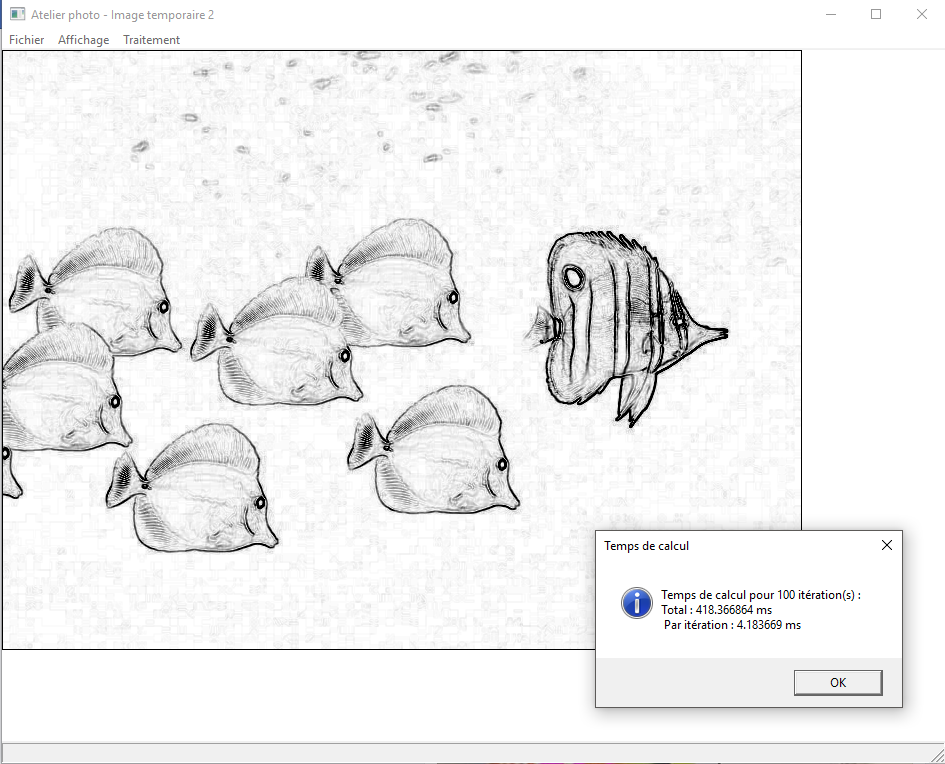
\includegraphics[scale=0.4]{26552611_10215381438792953_598457361_n.png}
\caption{Résultat du programme en assembleur de détection de contours}
\label{}
\end{figure}



Avec le code en C, pour 100 itérations on obtient 12,24ms par itérations, on voit donc que le code en assembleur est nettement plus rapide que le code en C. 


\end{document}
